\chapter{Introduction}

\section{Terminology}
\begin{itemize}

\item Browser extension -- third party code that is integrated with the browser API-s.

\item Certificate -- a file that binds the public key with the identity of the key owner. In this document, we are only considering certificates that are issued by certificate authorities.

\item Certificate authority (CA) -- a trusted third party, who issues certificates to end users (citizens or organisations) or assigns trust to lower level certificate authorities.

\item eID -- electronic identification, a digital solution for proof of identity of citizens or organisations.

\item Local attacker -- an attacker who has either physical or remote access to the user's computer.

\item Local attacker with administrative permissions -- an attacker who can do everything that the administrator can do. Such an attacker can be considered to control the whole computer, including what is displayed on the screen.

\item Local attacker with user permissions -- an attacker who does not have access to functionalities that require administrative permissions. Such an attacker can perform unprivileged system calls, which can differ depending on the operating system.

\item Man-in-the-middle attack (MITM) -- an attack where the attacker relays messages between two parties. Thus an attacker can eavesdrop and modify the exchanged messages.

\item Powerful attacker -- an attacker who can get a valid certificate for a selected domain and who is also able to perform DNS spoofing. This would enable running a man-in-the-middle attack.

\item Service provider -- the party who is running the web service / server application that provides the option for the client to authenticate or issue digital signatures by using the new browser extension.

\item TLS -- Transport Layer Security, a cryptographic protocol for secure Internet communication.

\item OCSP -- Online Certificate Status Protocol, an Internet protocol used for obtaining the revocation status of a X.509 digital certificate.

\item Web service -- the service which the client is authenticating to or which asks the client to give a digital signature with the Web eID browser extension.


\end{itemize}

\section{The scope of the analysis}
\label{sec:scope}
The new browser extension allows the web services to authenticate users and ask them to issue signatures. Thus, the main scope of the analysis contains the browser, native Web eID application, the service provider and their interaction (see Figure~\ref{fig:scope}).

\begin{figure}[ht]
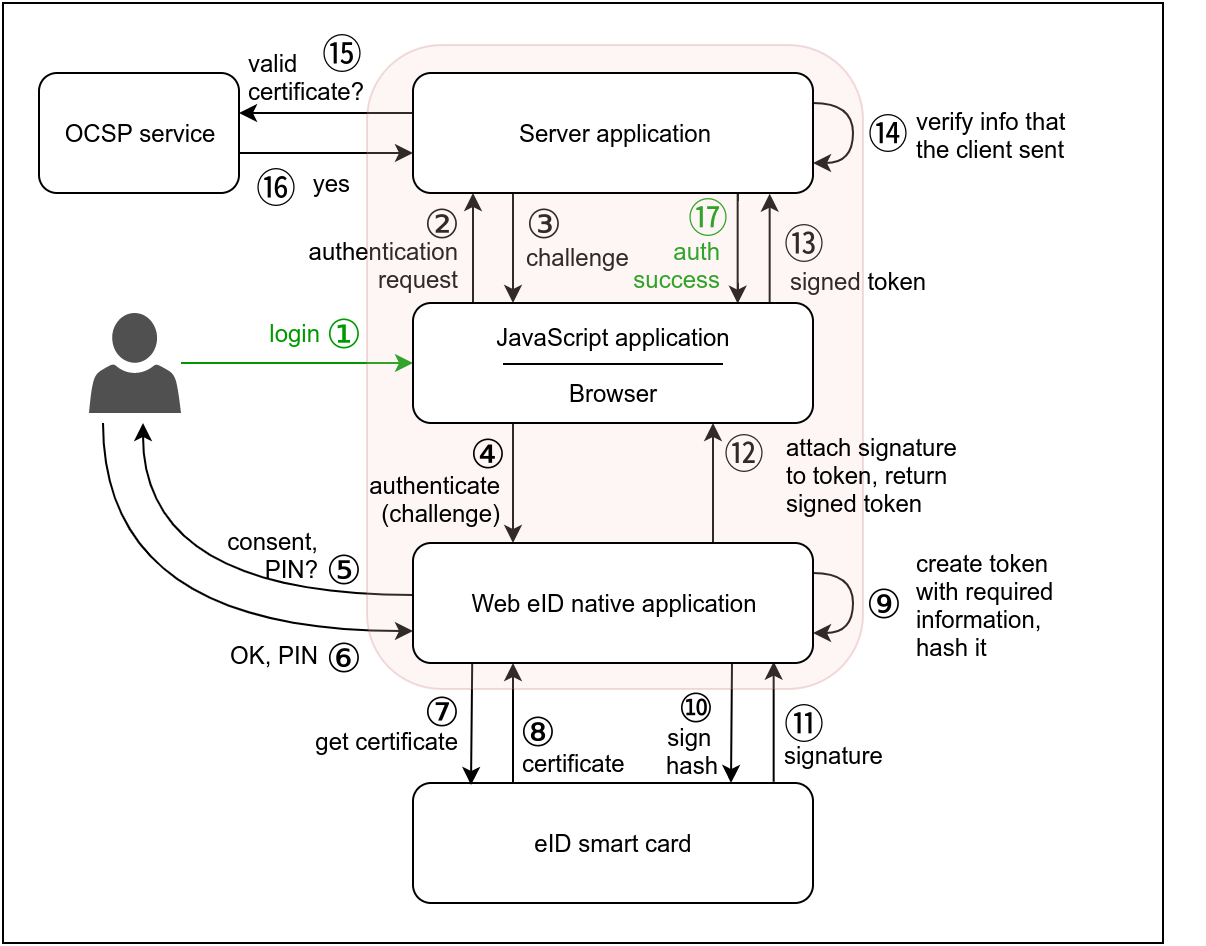
\includegraphics[width=\columnwidth]{img/main_scope_1.png}
\caption{The main scope of the current analysis is highlighted and covers the interaction between the server application, browser and native Web eID application. The  authentication and signing protocols are described in the  Web eID architecture draft: \url{https://github.com/open-eid/browser-extensions2}.}
\label{fig:scope}
\end{figure}

However, security of the new architecture also depends on multiple external factors that are not in the main scope, so at times we also need to talk about the extended scope.

For example, the user's device has to be trusted to behave correctly. It is difficult to protect user's digital identity while the device is infected and controlled by malware. Therefore, protecting user environment is mostly the responsibility of the user or the corresponding organisation. Although there are technologies that can protect the user in a malicious environment, they usually rely on additional hardware. Providing additional hardware for the end users is out of the scope of this project. Still, it may also be possible to apply software based mitigation measures to make it more difficult to attack the user environment. For example, an attack is more difficult if it requires superuser permissions.

In addition, the certificate authorities that issue eID certificates and TLS certificates for web services have to be trusted. The CA has to protect its signing key from third parties to prevent it being misused to issue fraudulent certificates. The CA also has to properly authenticate the party who is requesting a certificate. There are specific requirements which the certificate authorities have to follow. The security of the CA-s is out of the scope of this project. Thus, we assume that the certificate authorities behave according to their requirements and that they are properly audited.

Although the main scope of this analysis does not cover the CA-s and the local computer, the approach that we chose for the analysis tries to list all the relevant threats that could affect the security of authentication or signing in the new architecture. Therefore, we also list threats caused by entities that are out of scope of the Web eID architecture. Based on this information, the overall threat landscape can be seen. While the mitigation of external threats is not in the scope of this project, these threats could be mitigated by organisational measures or by third parties who are responsible for the corresponding components.

We recommend to conduct a follow-up study to investigate the threats to the end user from an untrusted computing device. It is important to understand how a compromised local machine can be abused depending on which level of access the attacker has to the system. As different operating systems have different API-s and permission systems, this study should be performed for each supported operating system.

\section{Security objectives and requirements}

\subsection{Security of authentication}

On a high level, authentication protocols need to achieve the following properties to be considered secure~\cite{BoMa10}.

\begin{labeling}{Entity authentication:}
    \item[Entity authentication:] the service provider obtains a reasonable level of assurance that the entity requesting authentication is who they claim to be.
    \item[Freshness:] the service provider obtains a reasonable level of assurance that the authentication request is recent.
\end{labeling}

Typically, we want the authentication to be \emph{mutual}, i.e. we also require the following property.

\begin{labeling}{Origin authentication:}
    \item[Origin authentication:] the user obtains a reasonable level of assurance that the service he/she is authenticating to is who they claim to be.
\end{labeling}

In order to satisfy these requirements, several lower level properties must hold.

\begin{labeling}{Impersonation resistance:}
    \item[Credential validity:] it must be possible to establish whether the credentials used for authentication are valid.
    \item[Authorised usage:] it must be hard to use the credentials in an unauthorised manner.
    \item[Impersonation resistance:] the protocol should provide reasonable level of assurance against malicious impersonation attacks (e.g. man-in-the-middle and session hijacking). 
    \item[Cryptographic strength:] the algorithms in use must withstand the attempts to violate the cryptographic properties. 
\end{labeling}

\subsection{Security of signing}

On a high level, signature protocols need to achieve the following properties to be considered secure.

\begin{labeling}{Entity authentication:}
    \item[Entity authentication:] the signature should identify the signing person/entity with high level of assurance.
    \item[Non-repudiation:] the entity who has given the signature is unable to deny neither the fact of signing, nor the knowledge of the signed content (together with all its possible binding implications) after the fact. 
    \item[Data integrity:] the party verifying the signature gets assurance that the data under the signature has not been changed between the moments of signing and verification.
\end{labeling}

In order to satisfy these requirements, several lower level properties must hold.

\begin{labeling}{Cryptographic strength:}
    \item[Credential validity:] it must be possible to establish whether the credentials used for signing were valid at the time of signing.
    \item[Authorised usage:] it must be hard to use the credentials in an unauthorised manner.
    \item[Cryptographic strength:] the algorithms in use must withstand the attempts to violate the cryptographic properties.
\end{labeling}

